\subsection{Геометрические алгоритмы}
\subsubsection{Линейная интерполяция}
\begin{figure}[h!]
\centering
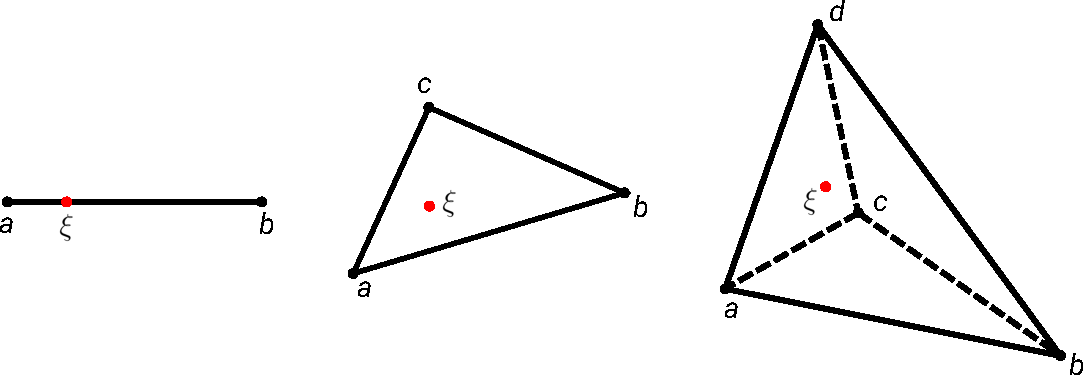
\includegraphics[width=0.8\linewidth]{geom_interp.pdf}
\caption{Порядок нумерации точек одномерного, двумерного и трёхмерного симплекса при линейной интерполяции}
\label{fig:geom_interp}
\end{figure}
Пусть функция $u$ задана в узлах симплекса, имеющего нумерацию согласно рис.~\ref{fig:geom_interp}.
Необходимо найти значение этой функции в точке $\vec \xi$ (эта точка вообще говоря не обязана лежать внутри симлекса).

Интерполяция в одномерном, двумерном и трёхмерном виде запишется как
\begin{align}
\label{eq:simplex_interp_1d}
&u(\xi) =
\frac{
|\triangle_{\xi a}|u(b)+
|\triangle_{b \xi}|u(a)
}
{|\triangle_{ba}|}
\\[10pt]
\label{eq:simplex_interp_2d}
&u(\xi) =
\frac{
|\triangle_{ab\xi}|u(c) +
|\triangle_{bc\xi}|u(a) +
|\triangle_{ca\xi}|u(b)
}
{|\triangle_{abc}|}
\\[10pt]
\label{eq:simplex_interp_3d}
&u(\xi) =
\frac{
|\triangle_{abc\xi}|u(d) +
|\triangle_{cbd\xi}|u(a) +
|\triangle_{cda\xi}|u(b) +
|\triangle_{adb\xi}|u(c)
}
{|\triangle_{abcd}|},
\end{align}
где $|\triangle|$ -- знаковый объём симплекса, вычисляемый как
\begin{align*}
& |\triangle_{ab}| = b - a, \\[10pt]
& |\triangle_{abc}| = \left(\frac{(\vec b - \vec a)\times(\vec c - \vec a)}{2}\right)_z, \\[10pt]
& |\triangle_{abcd}| = \frac{(\vec b - \vec a)\cdot\left((\vec c - \vec a)\times(\vec d - \vec a)\right)}{6}.\\[10pt]
\end{align*}

\subsubsection{Преобразование координат}
\label{sec:coo_transform} 
Рассмотрим преобразование
из двумерной параметрической системы координат $\vec \xi$ 
в физическую систему $\vec x$.
Такое преобразование полностью определяется покоординатными
функциями $\vec x(\vec \xi)$.
Далее получим соотношения, связывающие операции дифференцирования
и интегрирования в физической и параметрической областях.

\subsubsubsection{Матрица Якоби}
Будем рассматривать двумерное преобразование $(\xi, \eta) \to (x, y)$.
Линеаризуем это преобразование (разложим в ряд Фурье до линейного слагаемого)
\begin{align*}
& x(\xi_0 + d\xi, \eta_0 + d\eta) \approx x_0 + \left.\dfr{x}{\xi}\right|_{\xi_0, \eta_0} d\xi
    + \left.\dfr{x}{\eta}\right|_{\xi_0, \eta_0} d\eta, \\
& y(\xi_0 + d\xi, \eta_0 + d\eta) \approx y_0 + \left.\dfr{y}{\xi}\right|_{\xi_0, \eta_0} d\xi
    + \left.\dfr{y}{\eta}\right|_{\xi_0, \eta_0} d\eta,
\end{align*}
где $x_0 = x(\xi_0, \eta_0)$, $y_0 = y(\xi_0, \eta_0)$.
Переписывая это выражение в векторном виде, получим
\begin{equation}
\label{eq:jacobi_linear}
\vec{x}(\vec \xi_0 + \vec{d\xi} ) - \vec{x}_0 = J(\vec \xi_0) \; \vec{d\xi}.
\end{equation}
Матрица $J$ (зависящая от точки приложения в параметрической плоскости) называется матрицей Якоби:
\begin{equation}
\label{eq:jacobi_matrix_2d}
J = \left(
	\begin{array}{cc}
	J_{11} & J_{12}\\[10pt]
	J_{21} & J_{22}\\
	\end{array}
\right)
= \left(
	\begin{array}{cc}
	\ddfr{x}{\xi} & \ddfr{x}{\eta}\\[10pt]
	\ddfr{y}{\xi} & \ddfr{y}{\eta}\\
	\end{array}
\right)
\end{equation}

\paragraph{Якобиан}

\begin{figure}[h!]
\centering
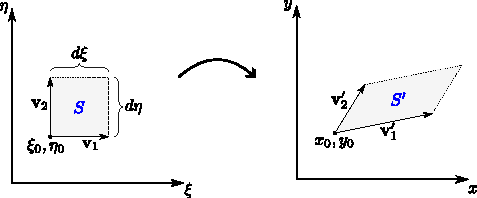
\includegraphics[width=0.6\linewidth]{dxideta.pdf}
\caption{Преобразование элементарного объёма}
\label{fig:dxideta}
\end{figure}

Определитель матрицы Якоби (якобиан), взятый в конкретной точке параметрической плоскости $\vec\xi_0$, показывает,
во сколько раз увеличился элементарный объём около этой точки в результате преобразования.
Действительно, рассмотрим два перпендикулярных элементарных вектора
в параметрической системе координат: $\vec v_1 = (d\xi, 0)$ и $\vec v_2 = (0, d\eta)$
отложенных от точки $\vec\xi_0$ (см.~\figref{fig:dxideta}).
В результате преобразования по формуле \cref{eq:jacobi_linear} 
получим следующие преобразования концевых точек и векторов:
\begin{align*}
& (\xi_0, \eta_0) \to (x_0, y_0), \\
& (\xi_0 + d\xi, \eta_0) \to (x_0 + J_{11} d\xi, y_0 + J_{21} d\xi) \hence \vec v_1 \to \vec v'_1 = (J_{11} d\xi, J_{21} d\xi), \\
& (\xi_0 , \eta_0 + d\eta) \to (x_0 + J_{12} d\eta, y_0 + J_{22} d\eta) \hence \vec v_2 \to \vec v'_2 = (J_{12} d\eta, J_{22} d\eta).
\end{align*}
Элементарный объём равен площади параллелограмма, построенного
на элементарных векторах.
В параметрической плоскости согласно \cref{eq:vec_cross_2d} получим 
$$ |S| = \vec v_1 \times \vec v_2 = d\xi d\eta,$$
и аналогично для физической плоскости:
$$
|S'| = \vec v'_1 \times \vec v'_2 = (J_{11} J_{22} - J_{12} J_{21})d\xi d\eta = |J| d\xi d\eta
$$
Сравнивая два последних соотношения приходим к выводу,
что элементарный объём в результате преобразования увеличился в $|J|$ раз. Тогда можно записать
\begin{equation}
\label{eq:dxdy_dxideta}
dx\,dy = |J|\,d\xi\,d\eta
\end{equation}

Многомерным обобщением этой формулы будет
\begin{equation}
\label{eq:vec_dx_dxi}
d\vec x = |J|\,d\vec \xi
\end{equation}

\subsubsubsection{Дифференцирование в параметрической плоскости}
Пусть задана некоторая функция $f(x, y)$. Распишем её производную по
параметрическим координатам:
\begin{align*}
&\dfr{f}{\xi} = \dfr{f}{x}\dfr{x}{\xi} + \dfr{f}{y}\dfr{y}{\xi}, \\
&\dfr{f}{\eta} = \dfr{f}{x}\dfr{x}{\eta} + \dfr{f}{y}\dfr{y}{\eta}.
\end{align*}
Вспоминая определение \cref{eq:jacobi_matrix_2d}, запишем
\begin{equation*}
\left(\begin{array}{c}
  \ddfr{f}{\xi} \\[10pt]
  \ddfr{f}{\eta}
  \end{array}
\right) = 
J^T 
\left(
  \begin{array}{c}
  \ddfr{f}{x} \\[10pt]
  \ddfr{f}{y}
  \end{array}
\right) =
\left(
  \begin{array}{cc}
    J_{11} & J_{21} \\[10pt]
    J_{12} & J_{22}
  \end{array}
\right)
\left(
  \begin{array}{c}
  \ddfr{f}{\xi} \\[10pt]
  \ddfr{f}{\eta}
  \end{array}
\right)
\end{equation*}
Обратная зависимость примет вид
\begin{equation*}
\left(\begin{array}{c}
  \ddfr{f}{x} \\[10pt]
  \ddfr{f}{y}
  \end{array}
\right) = 
\left(J^T\right)^{-1}
\left(
  \begin{array}{c}
  \ddfr{f}{\xi} \\[10pt]
  \ddfr{f}{\eta}
  \end{array}
\right) =
\frac{1}{|J|}
\left(
  \begin{array}{cc}
    J_{22} & -J_{21} \\[10pt]
    -J_{12} & J_{11}
  \end{array}
\right)
\left(
  \begin{array}{c}
  \ddfr{f}{\xi} \\[10pt]
  \ddfr{f}{\eta}
  \end{array}
\right)
\end{equation*}
В многомерном виде запишем
\begin{equation}
\label{eq:vec_grad_dx}
\nabla_{\vec x} f = \left(J^T\right)^{-1} \nabla_{\vec \xi} f.
\end{equation}

\subsubsubsection{Интегрирование в параметрической плоскости}
Пусть в физической области $\vec x$ задана область $D_x$.
Интеграл функции $f(\vec x)$ по этой области
можно расписать, используя замену \cref{eq:vec_dx_dxi}
\begin{equation}
\label{eq:dxideta_integral}
\int\limits_{D_{x}}f(\vec x)\,d\vec x = \int\limits_{D_{\xi}}f(\vec \xi) \, |J(\vec \xi)|d\vec \xi,
\end{equation}
где $f(\vec \xi) = f(\vec x(\vec \xi))$, а $D_\xi$ -- образ области $D_x$ в параметрической плоскости.

\subsubsubsection{Двумерное линейное преобразование. Параметрический треугольник}
\label{sec:lintri_transform}
\begin{figure}[h!]
\centering
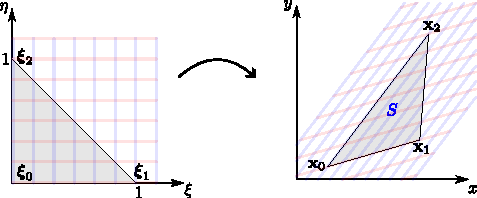
\includegraphics[width=0.6\linewidth]{lintri_transform.pdf}
\caption{Преобразование из параметрического треугольника}
\label{fig:lintri_transform}
\end{figure}
Рассмотрим двумерное преобразование, при котором
определяющие функции являются линейными. То есть представимыми в виде
\begin{align*}
x(\xi, \eta) = A_x \xi + B_x \eta + C_x, \\
y(\xi, \eta) = A_y \xi + B_y \eta + C_y.
\end{align*}
Для определения шести констант, определяющих это преобразование,
достаточно выбрать три любые (не лежащие на одной прямой) точки:
$(\xi_i, \eta_i) \to (x_i, y_i)$ для $i=0,1,2$.
В результате получим систему из шести линейных уравнений (три точки по две координаты),
из которой находятся конcтанты $A_{x,y}, B_{x,y}, C_{x,y}$.
Пусть три точки в параметрической плоскости
образуют единичный прямоугольный треугольник (\figref{fig:lintri_transform}):
\begin{equation*}
\xi_0, \eta_0 = (0, 0),\quad
\xi_1, \eta_1 = (1, 0),\quad
\xi_2, \eta_2 = (0, 1).
\end{equation*}
Тогда система линейных уравнений примет вид
\begin{align*}
&x_0 = C_x,       \quad y_0 = C_y, \\
&x_1 = A_x + C_x, \quad y_1 = A_y + C_y, \\
&y_2 = B_x + C_x, \quad y_2 = B_y + C_y.
\end{align*}
Определив коэффициенты преобразования их этой системы, окончательно запишем преобразование
\begin{equation}
\label{eq:lintri_transform}
\begin{aligned}
&x(\xi, \eta) = (x_1 - x_0)\xi + (x_2 - x_0) \eta + x_0,\\
&y(\xi, \eta) = (y_1 - y_0)\xi + (y_2 - y_0) \eta + y_0.\\
\end{aligned}
\end{equation}
Матрица Якоби этого преобразования \cref{eq:jacobi_matrix_2d}
не будет зависеть от параметрических координат $\xi, \eta$:
\begin{equation}
\label{eq:lintri_jacobi_matrix}
J = \left(
\begin{array}{cc}
x_1 - x_0 & x_2 - x_0 \\
y_1 - y_0 & y_2 - y_0 \\
\end{array}
\right).
\end{equation}
Якобиан преобразования будет равен удвоенной площади треугольника $S$, составленного из определяющих точек в физической плоскости:
\begin{equation}
\label{eq:lintri_jacobian}
|J| = (x_1 - x_0) (y_2 - y_0) - (y_1 - y_0) (x_2 - x_0) = (\vec x_1 - \vec x_0) \times (\vec x_2 - \vec x_0) = 2 |S|.
\end{equation}
Распишем интеграл по треугольнику $S$ по формуле \cref{eq:dxideta_integral}.
Вследствии линейности преобразования якобиан постоянен и, поэтому, его можно вынести его из-под интеграла:
\begin{equation}
\label{eq:lintri_integral}
\int\limits_{S}f(x, y)\,dxdy = |J|\int\limits_0^1 \int\limits_0^{1-\xi} f(\xi, \eta) d\eta d\xi.
\end{equation}

\subsubsubsection{Двумерное билинейное преобразование. Параметрический квадрат}
\label{sec:bilinquad_transform}
\begin{figure}[h!]
\centering
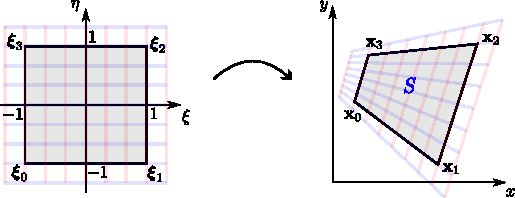
\includegraphics[width=0.6\linewidth]{bilinquad_transform.pdf}
\caption{Преобразование из параметрического квадрата}
\label{fig:bilinquad_transform}
\end{figure}

\subsubsubsection{Трёхмерное линейное преобразование. Параметрический тетраэдр}
TODO

\subsubsection{Свойства многоугольника}
\subsubsubsection{Площадь многоугольника}
\label{sec:polygon_area} 

\begin{figure}[h!]
\centering
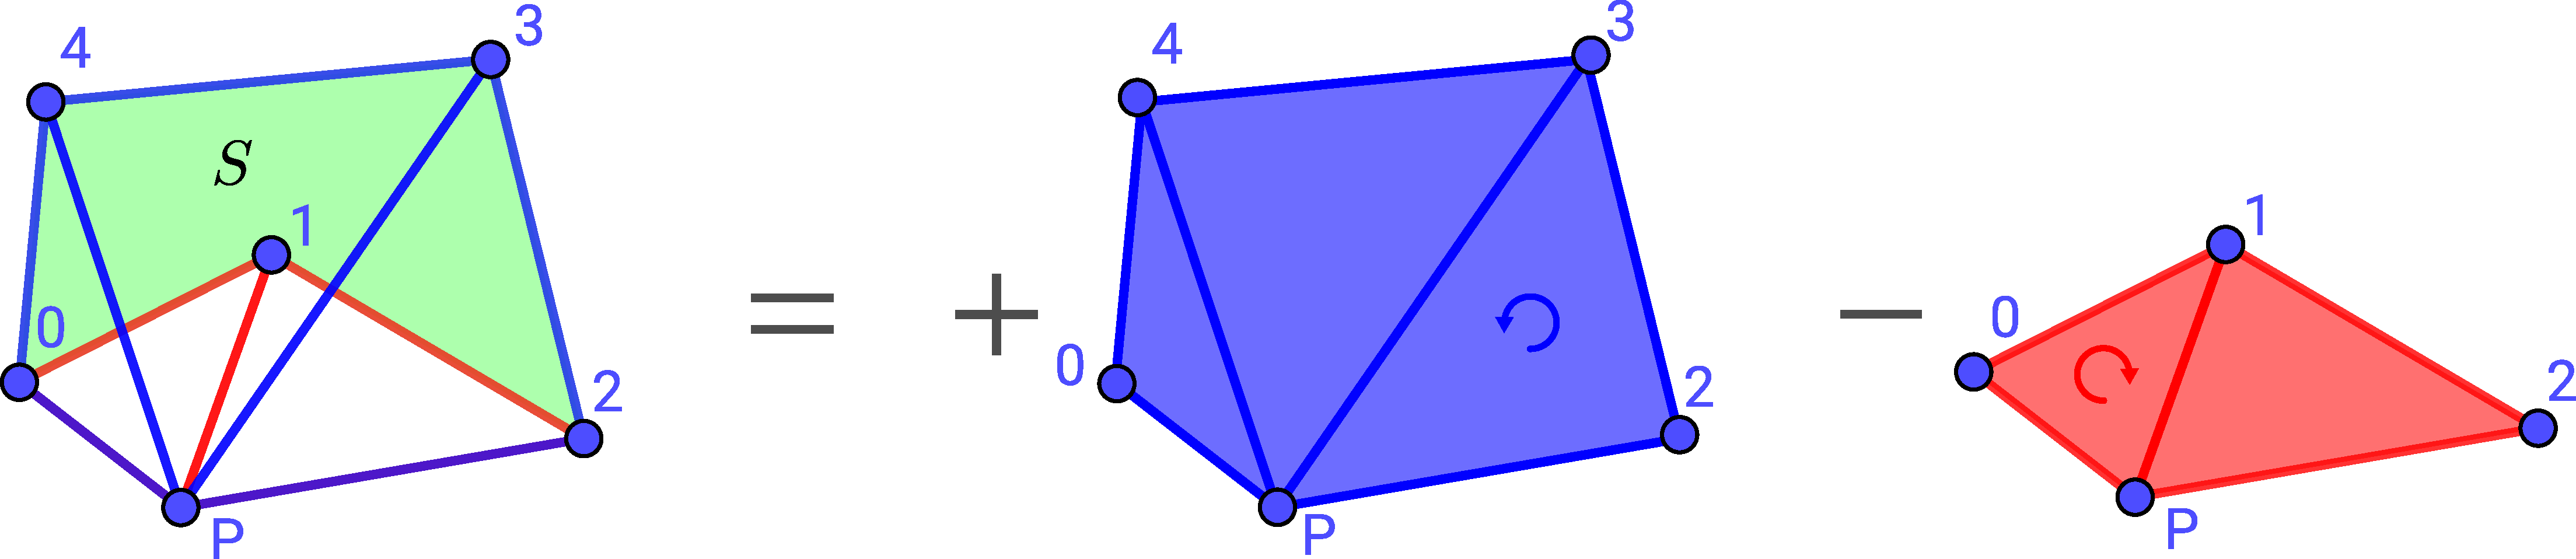
\includegraphics[width=0.7\linewidth]{polygon_area.pdf}
\caption{Площадь произвольного многоугольника}
\label{fig:polygon_area}
\end{figure}

Рассмотрим произвольный несамопересекающийся $N$-угольник $S$,
заданный координатами своих узлов $\vec x_i$, $i=\overline{0, N-1}$,
пронумерованных последовательно против часовой стрелки (\figref{fig:polygon_area}).
Далее введём произвольную точку $\vec p$ и 
от этой точки будем строить ориентированные треугольники до граней многоугольника:
$$
\triangle^p_i = (\vec p, \vec x_i, \vec x_{i+1}), \quad i=\overline{0, N-1},
$$
(для корректности записи будем считать, что $\vec x_N = \vec x_0$).
Тогда площадь исходного многоугольника $S$ будет равна сумме
знаковых площадей треугольников $\triangle^p_i$:
$$
|S| = \sum_{i=0}^{N-1} |\triangle^p_i|, \qquad |\triangle^p_i| = \frac{(\vec x_i - \vec p) \times (\vec x_{i+1} - \vec p)}{2}.
$$
Знак площади ориентированного треугольника зависит от направления закрутки его узлов:
она положительна для закрутки против часовой стрелки и отрицательна, если узлы пронумерованы по часовой стрелке.
В частности, на рисунке~\ref{fig:polygon_area} видно, что треугольники, отмеченные красным: $P01, P12$, будут
иметь отрицательную площадь, а синие треугольники $P23$, $P34$, $P40$ -- положительную. Сумма этих площадей
с учётом знака даст искомую площадь многоугольника.

Для сокращения вычислений воспользуемся произвольностью положения $\vec p$ и совместим
её с точкой $\vec x_0$. Тогда треугольники $\triangle^p_0$, $\triangle^p_{N-1}$
выродятся (будут иметь нулевую площадь).
Обозначим такую последовательную триангуляцию как
\begin{equation}
\label{eq:seq_polygon_triangulation}
\triangle_i = (\vec x_0, \vec x_i, \vec x_{i+1}), \qquad i=\overline{1,N-2}.
\end{equation}
Знаковая площадь ориентированного треугольника будет равна
\begin{equation}
\label{eq:seq_triangle_area}
|\triangle_i| = \frac{(\vec x_i - \vec x_0) \times (\vec x_{i+1} - \vec x_0)}{2}.
\end{equation}
Тогда окончательно формула определения площади примет вид
\begin{equation}
\label{eq:polygon_area}
|S| = \sum_{i=1}^{N-2}|\triangle_i|.
\end{equation}

\paragraph{Плоский полигон в пространтве} Если плоский полигон $S$ расположен в трёхмерном пространстве,
то правая часть формулы \cref{eq:seq_triangle_area} согласно определению векторного произведения в трёхмерном пространстве \cref{eq:vec_cross}
-- есть вектор.
Чтобы получить скалярную площадь, нужно спроецировать этот вектор на единичную нормаль к плоскости
многоугольника:
$$
\vec n = \frac{\vec k}{|\vec k|}, \qquad \vec k = (\vec x_1 - \vec x_0) \times (\vec x_2 - \vec x_0).
$$
Эта формула записана из предположения, что узел $\vec x_2$ не лежит
на одной прямой с узлами $\vec x_0$, $\vec x_1$. Иначе вместо $\vec x_2$ нужно
выбрать любой другой узел, удовлетворяющий этому условию.
Тогда площадь ориентированного треугольника, построенного
в трёхмерном пространстве запишется через смешанное произведение:
\begin{equation}
\label{eq:seq_triangle_area_3d}
|\triangle_i| = \frac{\left((\vec x_i - \vec x_0) \times (\vec x_{i+1} - \vec x_0) \right)\cdot \vec n}{2}.
\end{equation}
Формула для определения площади полигона \cref{eq:polygon_area} будет по прежнему верна.
При этом итоговый знак величины $S$ будет положительным,
если закрутка полигона положительная (против часовой стрелки) при взгляде со стороны
вычисленной нормали $\vec n$.

\subsubsubsection{Интеграл по многоугольнику}
\label{sec:polygon_integral} 
Рассмотрим интеграл функции $f(x,y)$ по $N$-угольнику $S$, заданному последовательными координатами своих узлов $\vec x_i$.
Введём последовательную триангуляцию согласно \cref{eq:seq_polygon_triangulation}.
Тогда интеграл по многоугольнику можно расписать как сумму интегралов по ориентированным треугольникам:
\begin{equation}
\label{eq:seq_triangulation_integral}
\arint{f(x,y)}{S}{xdy} = \sum_{i=1}^{N-2} \arint{f(x,y)}{\triangle_i}{xdy}.
\end{equation}
Далее для вычисления интегралов в правой части
воспользуемся преобразованием к параметрическому треугольнику (п.~\ref{sec:lintri_transform}).
Следуя формуле интегрирования \cref{eq:lintri_integral}, распишем
интеграл по $i$-ому треугольнику:
\begin{equation*}
\arint{f(x,y)}{\triangle_i}{xdy} = |J_i| \int\limits_{0}^{1}\int\limits_{0}^{1-\xi} f_i(\xi, \eta) \, d\eta d\xi,
\end{equation*}
где якобиан $|J_i|$ согласно \cref{eq:lintri_jacobian} есть удвоенная площадь ориентированного треугольника $\triangle_i$
(положительная при закрутке против часовой стрелке и отрицаетельная иначе):
\begin{equation*}
|J_i| = 2|\triangle_i| = (\vec x_i - \vec x_0) \times (\vec x_{i+1} - \vec x_0),
\end{equation*}
а функция $f_i(\xi, \eta)$ есть функция от преобразованных согласно \cref{eq:lintri_transform}
переменных:
\begin{equation*}
f_i(\xi, \eta) = f\left(\left(\vec x_i - \vec x_0\right)\xi + \left(\vec x_{i+1} - \vec x_0\right)\eta + \vec x_0\right).
\end{equation*}
Окончательно запишем
\begin{equation}
\label{eq:polygon_integral}
\arint{f(x,y)}{S}{xdy} = 2 \sum_{i=1}^{N-2}
    |\triangle_i| \int\limits_{0}^{1}\int\limits_{0}^{1-\xi} f_i(\xi, \eta) \, d\eta d\xi.
\end{equation}
Отметим, что эта формула работает и в том случае, когда
полигон расположен в трёхмерном пространстве
(знаковую площадь при этом следует вычислять по \cref{eq:seq_triangle_area_3d}).

\subsubsubsection{Центр масс многоугольника}
\label{sec:polygon_center} 
По определению, координаты центра масс $\vec c$ области $S$ равны среднеинтегральным значениям координатных функций. То есть
\begin{equation*}
c_x = \frac{1}{|S|}\int\limits_{S} x \, dxdy,
\quad 
c_y = \frac{1}{|S|}\int\limits_{S} y \, dxdy.
\end{equation*}
Далее распишем интеграл в правой части через последовательную триангуляцию согласно
\cref{eq:seq_triangulation_integral} с учётом линейного преобразования
\cref{eq:lintri_transform}:
\begin{align*}
\int\limits_{S} x \, dxdy &= \sum_{i=1}^{N-2} \int\limits_{\triangle_i} x \, dxdy\\
                          &= \sum_{i=1}^{N-2} |J_i| \int\limits_0^1\int\limits_0^{1-\xi} ((x_i - x_0)\xi + (x_{i+1} - x_0)\eta + x_0)\, d\eta d\xi\\
                          &= \sum_{i=1}^{N-2} \frac{|J_i|}{2}\frac{x_0 + x_i + x_{i+1}}{3}\\
                          &= \sum_{i=1}^{N-2} |\triangle_i|\frac{x_0 + x_i + x_{i+1}}{3}.
\end{align*}
Итого, с учётом \cref{eq:polygon_area}, координаты центра масс примут вид
\begin{align*}
&\vec c = \dfrac{\displaystyle\sum_{i=1}^{N-2} \dfrac{\vec x_0 + \vec x_i + \vec x_{i+1}}{3}|\triangle_i|}{\displaystyle\sum_{i=1}^{N-2} |\triangle_i|}.
\end{align*}
Если полигон расположен в двумерном пространстве $xy$, то знаковая площадь треугольников
вычисляется по формуле \cref{eq:seq_triangle_area}.
В случае трёхмерного пространтва должна использоваться формула \cref{eq:seq_triangle_area_3d}.

\subsubsection{Свойства многогранника}
\subsubsubsection{Объём многогранника}
\label{sec:polyhedron_volume} 
TODO
\subsubsubsection{Интеграл по многограннику}
\label{sec:polyhedron_integral} 
TODO
\subsubsubsection{Центр масс многогранника}
\label{sec:polyhedron_center} 
TODO

\subsubsection{Поиск многоугольника, содержащего заданную точку}
TODO
